\documentclass[presentation]{beamer}
\usetheme{CambridgeUS}
\usecolortheme{orchid}

\definecolor{themeColor}{HTML}{1dc600}

\setbeamercolor*{structure}{bg=black,fg=themeColor}

\setbeamercolor*{palette primary}{use=structure,fg=white,bg=structure.fg}
\setbeamercolor*{palette secondary}{use=structure,fg=white,bg=structure.fg!75}
\setbeamercolor*{palette tertiary}{use=structure,fg=white,bg=structure.fg!50!black}
\setbeamercolor*{palette quaternary}{fg=white,bg=black}

\setbeamercolor{section in toc}{fg=black,bg=white}
\setbeamercolor{alerted text}{use=structure,fg=structure.fg!50!black!80!black}

\setbeamercolor{titlelike}{parent=palette primary,fg=structure.fg!50!black}
\setbeamercolor{frametitle}{bg=structure.fg!10!white,fg=structure.fg!50!black!80!black}

\setbeamercolor*{titlelike}{parent=palette primary}

\usepackage[T1]{fontenc}
\usepackage[utf8]{inputenc}
\usepackage{amssymb}
\usepackage{graphicx}
\usepackage{subfigure}
\usepackage{multirow}
\usepackage{hhline}
\usepackage{amsfonts,amstext,amssymb,wasysym}
\usepackage{fancyvrb}
\usepackage{alltt}
\usepackage{textcomp}
\usepackage{url}
\usepackage{multimedia,pgf}
\usepackage{geometry}
\usepackage{minted}
\usepackage{bibentry}
\usepackage{framed}
\usepackage{pmboxdraw}
\usepackage{newunicodechar}
\newunicodechar{└}{\textSFii}
\newunicodechar{├}{\textSFviii}
\newunicodechar{─}{\textSFx}
\usepackage{cleveref}
\nobibliography*

\title[03 - Dependency Management]{\small{Developing, maintaining, and sharing software tools for research} \\
\normalsize{Enforce reproducibility: dependency management and build automation}}

\author[D. Pianini]{
Danilo Pianini\\
\texttt{{\footnotesize danilo.pianini@unibo.it}}}


\institute[UniBo]
{\textsc{Alma Mater Studiorum}---Universit\`a di Bologna}

\date[\today{}]{Ph.D. course in Data Science and Computation \\
\scriptsize \today{} - Bologna (Italy)
}

\pgfdeclareimage[height=0.625cm]{university-logo}{images/logo}
\logo{\pgfuseimage{university-logo}}

\newcommand{\codefile}[4]{
	\begin{block}{\texttt{#2}}
		\inputminted[fontsize=#3,linenos=true,breaklines=true]{#4}{"workspace/#1/#2"}
	\end{block}
}
\newcommand{\java}[3]{\codefile{#1}{#2}{#3}{java}}
\newcommand{\ccode}[3]{\codefile{#1}{#2}{#3}{c}}
\newcommand{\cpp}[3]{\codefile{#1}{#2}{#3}{cpp}}
\newcommand{\groovy}[3]{\codefile{#1}{#2}{#3}{groovy}}
\newcommand{\kotlin}[3]{\codefile{#1}{#2}{#3}{kotlin}}
\newcommand{\scala}[3]{\codefile{#1}{#2}{#3}{scala}}
\newcommand{\python}[3]{\codefile{#1}{#2}{#3}{python}}
\newcommand{\markdown}[3]{\codefile{#1}{#2}{#3}{markdown}}
\newcommand{\terminal}[3]{\codefile{#1}{#2}{#3}{text}}

\newcommand{\tinier}{\fontsize{4pt}{5pt}\selectfont}
\newcommand{\fnurl}[1]{\footnote{\url{#1}}}

\begin{document}

\AtBeginSubsection[]{%
  \begin{frame}<beamer>
    \frametitle{Outline}
    \tableofcontents[currentsection,currentsubsection]
  \end{frame}
  \addtocounter{framenumber}{-1}% If you don't want them to affect the slide number
}

%===============================================================================
\frame[label=coverpage]{\titlepage}
%===============================================================================

%===============================================================================
%===============================================================================
\section*{Outline}
%===============================================================================
%===============================================================================

\frame{\tableofcontents}

%===============================================================================
%===============================================================================


\section{Assigning version numbers}

\subsection{General problem}

\begin{frame}{Software versioning}
    The process of assigning a unique identifier to a unique state of some software
    \begin{itemize}
        \item Used to \textit{distinguish} different software states
        \item Used to \textit{refer to} different states of the same software
        \item The identifier is normally a sequence of alfanumeric numbers
        \item Those numbers can be separated by other symbols, most frequently dots, slashes, and dashes
        \item Assigning IDs in a predictable way could help gathering information on the software itself
    \end{itemize}
\end{frame}

\begin{frame}{Versioning levels}
    Versioning can happen at different levels and for different \textit{scopes}
    \begin{block}{Levels}
        \begin{itemize}
            \item Versioning system: very fine grained, typically generated, non progressive version ids
            \item Subproject or feature: more coarsely grained, often using codenames
            \item Release level
            \item Macro level (e.g. Python vs. Python3)
        \end{itemize}
    \end{block}
    \begin{block}{Scopes}
        \begin{itemize}
            \item Internal
            \begin{itemize}
                \item A specific development point
                \item Any subproject, feature, or milestone
            \end{itemize}
            \item External
            \begin{itemize}
                \item A specific public release of the software
                \item A specific public development stage of the software
            \end{itemize}
        \end{itemize}
    \end{block}
\end{frame}

\subsection{Approaches}

\begin{frame}{Code naming}
    The version is represented by a (usually pronounceable) word, short phrase or acronym
    \begin{itemize}
        \item With few exceptions, do not provide any direct information on the project (often by purpose)
        \item Very frequently used internally to refer to new features
        \item Often used to ``protect'' the corporation from information leaking
        \item Often changed to purposely create confusion
        \item Used to separate pre-release versions from final releases (e.g. Longhorn only became Windows Vista at the release)
        \item Often associated for \textit{commercial} reasons to other version numbers (e.g. Ubuntu 18.04 \underline{Bionic Beaver} or MacOS X 10.13.5 \underline{Sierra})
        \item Reasons for codenames are often \textit{political} and \textit{commercial} rather than technical
    \end{itemize}

\end{frame}

\begin{frame}{Date based}
    The version is represented by a string representing the release date
    \begin{itemize}
        \item Dates don't always match development rate
        \begin{itemize}
            \item A project may change more in a week than in a year
        \end{itemize}
        \item Useful for projects that are fast-paced (multiple releases per week)
        \item Useful as a companion for other versioning schemes
        \item Useful at the commercial level for clearly indicating the novelty (and the age) of a project (e.g. Windows 98, Office 2003)
    \end{itemize}
\end{frame}

\begin{frame}{Unary numbering}
    The version is represented by a string whose length grows at each version
    \begin{itemize}
        \item Rather idiosyncratic
        \item Only useful for project that reached maturity
        \begin{itemize}
            \item Extremely unlikely in today's software world
        \end{itemize}
        \item May lead to version length explosion
        \item Unsuitable for scientific / research projects
    \end{itemize}
\end{frame}

\begin{frame}{Degree of compatibility}
    The version is represented one or more sequences, separately incremented, that reflect incrementally widespread changes in the product
    \begin{itemize}
        \item Probably the most diffused
        \item Often used in conjunction with other techniques
        \item Often used badly (see the Linux kernel)
        \item Formal methodologies for applying it exist
        \item Sometimes instead of indicating API-level changes, the version may indicate user-level perceivable changes
        \begin{itemize}
            \item Very much depends on who are the customers
        \end{itemize}
    \end{itemize}
\end{frame}

\subsection{Real World}

\begin{frame}{Microsoft Windows versioning}
    Combination of all the techniques:
    \begin{itemize}
        \item Dates (Windows 9x, 2001)
        \item Codenames (NT, Vista, XP, Millenium Edition)
        \item Pre-release codenames (Longhorn)
        \item Dates for internal builds
        \item Incremental versions on multiple levels (e.g. Windows 95 is also MS-DOS 7.0 and Windows 4.00)
        \item Separation between ``commercial'' versions and ``actual'' ``versions''
        \begin{itemize}
            \item e.g., Windows 7 is actually Windows 6.1, and Windows 10 is actually Windows 6.4
            \item One future Windows may actually become Windows 7.0, clashing with the ``commercial'' version of an older product
        \end{itemize}
    \end{itemize}
    The proliferation and inconsistencies in the versioning led to some issues.
    \begin{itemize}
        \item Ever wondered why there is no Windows 9?
    \end{itemize}
\end{frame}

\begin{frame}{Ubuntu versioning}
    Association of a date in format YY.MM and a two word codename in form of Adjective AnimalName. Both the words of the codename begin with the same letter.
    \begin{itemize}
        \item Version number does not track changes
        \begin{itemize}
            \item The development is arguably linear
            \item But actually new versions may bring in substantial novelties, e.g. entirely new graphical environments
        \end{itemize}
        \item ``LTS'' can be optionally appended to identify ``Long Term Support'' versions
        \item Two versions of Ubuntu can be compared by date but also by the first letter of their codename
        \begin{itemize}
            \item ``Zesty Zapus'' is newer than ``Utopic Unicorn''
            \item Unfortunately, since there are a limited number of letters, ``Bionic Beaver'' is newer than ``Xenial Xerus'' and ``Zesty Zapus''
        \end{itemize}
    \end{itemize}
\end{frame}

\begin{frame}{Wine versioning}
    Formerly a pure date, in ISO format without hyphens, e.g. \texttt{20040505}. The project switched to a classic versioning in form of \texttt{major.minor}
    \begin{itemize}
        \item The change may give some headaches to dependency managers, since \texttt{20040505} is bigger than \texttt{3.9} and other subsequent versions.
        \item A \texttt{0.Date} format for initial development releases would have been advisable with hindsight
    \end{itemize}
\end{frame}

\begin{frame}{\TeX{} $\pi$-versioning}
    Purely unary numbering converging to $\pi$
    \begin{itemize}
        \item Current version (released in January 2004) is \texttt{3.14159265}
        \item Every time a new version is produced, a number from $\pi$ is added to the version string
        \item Sustainable just because \TeX{} is now extremely stable, and development is almost frozen
    \end{itemize}
    \begin{block}{}
        \begin{quote}
            At the time of my death, it is my intention that the then-current versions of \TeX{} [...] be forever left unchanged, except that the final version numbers to be reported in the ``banner'' lines of the programs should become: \mintinline{tex}{TeX, Version $\pi$} [...]. From that moment on, all ``bugs'' will be permanent ``features''.
        \end{quote}
        \begin{flushright}
            Donald E. Knuth \cite{Knuth1990tex}
        \end{flushright}
    \end{block}
\end{frame}

\begin{frame}{Semantic Versioning (SemVer)}
    Encodes version numbers and their change to convey meaning about the underlying code and what has been modified from one version to the next.
    \begin{itemize}
        \item Written in RFC-style\fnurl{https://semver.org/}
        \item No-retract
        \item Versioned using Semantic versioning
    \end{itemize}
\end{frame}
\begin{frame}[allowframebreaks]{SemVer: format \texttt{X.Y.Z[-P[+B]]} part}
    \begin{itemize}
        \item Software using Semantic Versioning MUST declare a public API. This API could be declared in the code itself or exist strictly in documentation. However it is done, it should be precise and comprehensive.
        \item Once a versioned package has been released, the contents of that version MUST NOT be modified. Any modifications MUST be released as a new version.
        \item A normal version number MUST take the form \texttt{X.Y.Z} where \texttt{X}, \texttt{Y}, and \texttt{Z} are non-negative integers, and MUST NOT contain leading zeroes. \texttt{X} is the major version, \texttt{Y} is the minor version, and \texttt{Z} is the patch version. Each element MUST increase numerically.
        \item Patch version \texttt{Z} MUST be incremented if only backwards compatible bug fixes are introduced. A bug fix is defined as an internal change that fixes incorrect behavior.
        \item Minor version \texttt{Y} MUST be incremented if new, backwards compatible functionality is introduced to the public API. It MUST be incremented if any public API functionality is marked as deprecated. It MAY be incremented if substantial new functionality or improvements are introduced within the private code. It MAY include patch level changes. Patch version MUST be reset to 0 when minor version is incremented.
        \item Major version \texttt{X} MUST be incremented if any backwards incompatible changes are introduced to the public API. It MAY include minor and patch level changes. Patch and minor version MUST be reset to 0 when major version is incremented.
        \item Major version zero (0.y.z) is for initial development. Anything may change at any time. The public API should not be considered stable.
        \item Version 1.0.0 defines the public API. The way in which the version number is incremented after this release is dependent on this public API and how it changes.
        \item A pre-release version MAY be denoted by appending a hyphen and a series of dot separated identifiers immediately following the patch version. Identifiers MUST comprise only ASCII alphanumerics and hyphen \texttt{[0-9A-Za-z-]}. Identifiers MUST NOT be empty. Numeric identifiers MUST NOT include leading zeroes. A pre-release version indicates that the version is unstable and might not satisfy the intended compatibility requirements as denoted by its associated normal version.
        \item Build metadata MAY be denoted by appending a plus sign and a series of dot separated identifiers immediately following the patch or pre-release version. Identifiers MUST comprise only ASCII alphanumerics and hyphen [0-9A-Za-z-].
    \end{itemize}
\end{frame}

\begin{frame}{Python Enhancement Proposal 440}
    Python software must be versioned as described in PEP440\fnurl{https://www.python.org/dev/peps/pep-0440/}
    \begin{itemize}
        \item Very flexible, but very complicated
        \item Superset of Semantic Versioning
        \item Ordering of release segments is mandated
    \end{itemize}
    \mintinline{text}{[N!]N(.N)*[{a|b|rc}N][.postN][.devN]}
    \begin{itemize}
        \item Epoch segment: \texttt{N!}
        \item \textbf{Mandatory Release segment}: \texttt{N(.N)*}
        \item Pre-release segment: \mintinline{text}{{a|b|rc}}
        \item Post-release segment: \texttt{.postN}
        \item Development release segment: \texttt{.devN}
    \end{itemize}
\end{frame}

\begin{frame}{Selecting a good methodology is important}
    Think before choosing a versioning schema, and then \textbf{be consistent}
    \begin{itemize}
        \item Adopting codenames makes sense if:
        \begin{itemize}
            \item You have a large team with several sub projects being developed concurrently
            \item You want to protect your codebase by talking in a less understandable manner
            \item You want to promote features or products and you need a human-appealing name
        \end{itemize}
        \item Using dates makes sense if:
        \begin{itemize}
            \item The development process is fast and steady
            \item Dates are a detail of a better versioned system
        \end{itemize}
        \item Unary numbering is strongly discouraged
        \item Semantic versioning is warmly recommended
        \begin{itemize}
            \item Can be integrated with the DVCS
            \item Dates can be added (e.g. in the + section)
            \item Codenames can be appended informally if needed
        \end{itemize}
    \end{itemize}
\end{frame}

\section{Select a proper license}

\subsection{General problem}

\begin{frame}{What is a license}
    A legal instrument used to regulate access, use, and redistribution of software
    \begin{itemize}
        \item You generally want to retain some guarantees on the software, e.g.:
        \begin{itemize}
            \item be recognized as the orignal creator;
            \item decide whether or not someone else can redistribute it
            \item decide under which circumstances the software can be used
            \item get paid if others use it
        \end{itemize}
        \item Law can change greatly among countries
        \begin{itemize}
            \item If you are not a lawyer, or you can't pay a lawyer, don't come up with your license
            \item A custom license is likely to be in conflict with the law of some countries
            \item Better choosing something proven to work
        \end{itemize}
    \end{itemize}
\end{frame}

\begin{frame}{Copyright vs. copyleft}
    \begin{block}{Copyright}
        Legal right that grants the creator of an original work exclusive rights for its use and (re)distribution
    \end{block}
    \begin{block}{Copyleft}
        Practice (not a legal right!) in which an author surrenders some, but not all, rights under copyright law.
        \begin{itemize}
            \item \textit{Strong} if all derived works inherit the copyleft license, \textit{weak} if some kinds of work may not inherit it
            \item \textit{Full} if all the parts of the work are distributed under the terms of the copyleft license, \texttt{partial} if only some parts are.
        \end{itemize}
    \end{block}
\end{frame}

\begin{frame}{Licensing vs. ownership}
    \begin{block}{Ownership}
        Possession of a copy of software. The possession implies right to use, even if such use implies a violation of the license (e.g. for making changes to the software, or making incidental copies).
    \end{block}
    \begin{block}{Licensing}
        The software is not sold, but merely ``licensed'', namely permitted to be used, under the conditions of a End-user license agreement (EULA).
        
        This schema, which prevents e.g. reselling, is currently being challenged at the EU level
    \end{block}
\end{frame}

\begin{frame}{Proprietary vs. Free}
    \begin{center}
        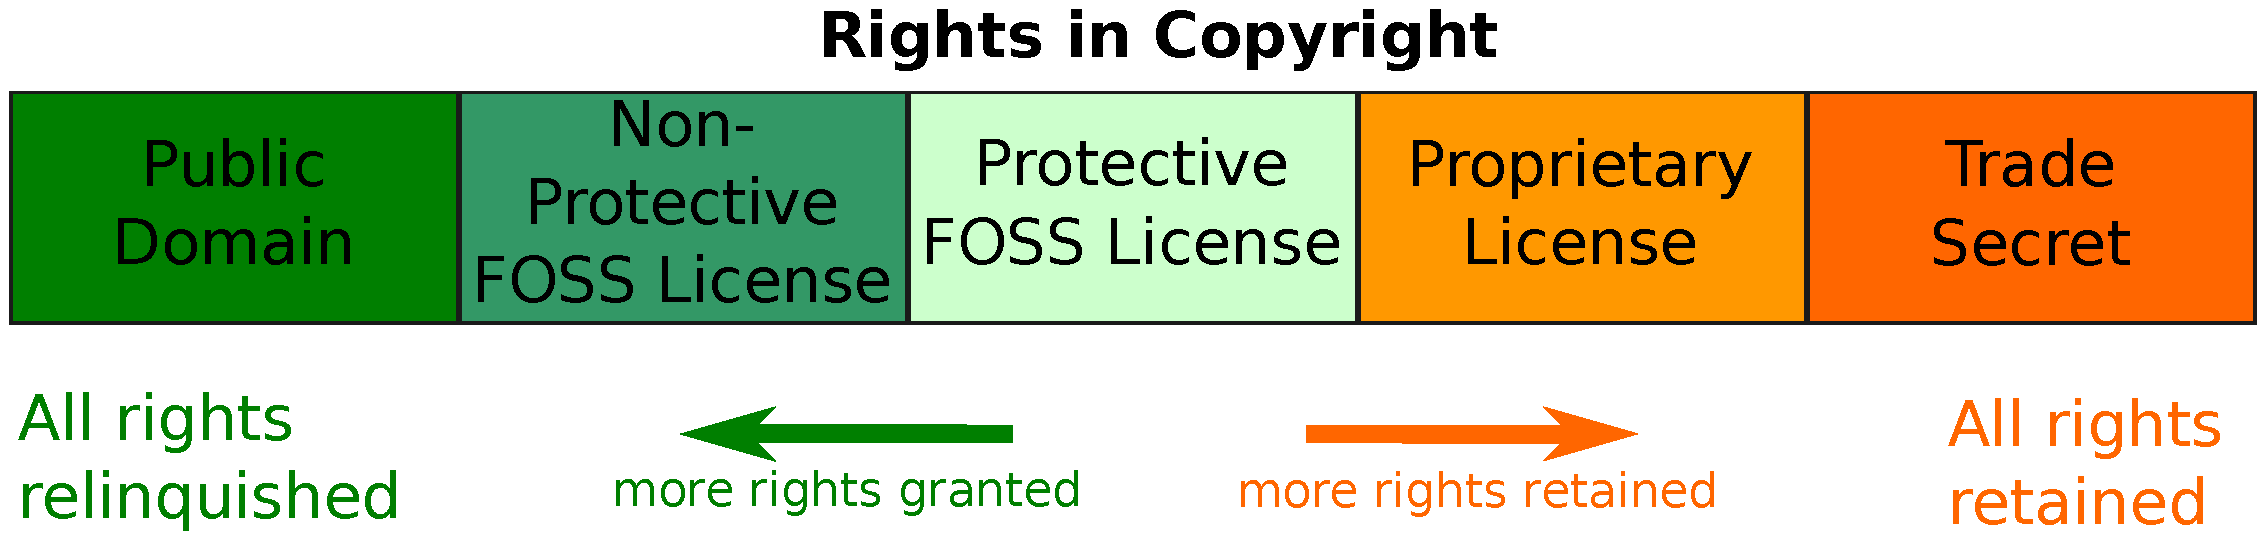
\includegraphics[width=\textwidth]{rights}
    \end{center}
    \vspace{-10pt}
    \begin{block}{Proprietary}
        The software publisher grants the right to use a certain number of copies under the conditions of an EULA, but does not transfer ownership of the copies to the customer. Usage of the software may be subjected to acceptance of the EULA.
    \end{block}
    \begin{block}{Free}
        The software publisher grants extensive rights to modify and redistribute the software, often prohibiting rolling back such rights (copyleft).
    \end{block}
\end{frame}

\begin{frame}{Free as in speech vs. free as in beer}
    Much easier for Italian speakers, as free is translated either with \textit{libero} (as in speech) or \textit{gratuito} (as in beer).
    \begin{block}{Free as in beer}
        The user pays nothing for using the software. It is free of charge.
    \end{block}
    \begin{block}{Free as in speech}
        The user receives the source code of the software, is allowed to modify it and redistribute it. The user can be asked to pay for receiving a copy: it can be distributed behind a fee. The author can also ask for additional money for accessing the source code (but not too much, asking for a billion dollars would let the software go back to the state of proprietary).
    \end{block}
\end{frame}

\begin{frame}{Free vs. Open source}
    They often go together, but they are different
    \begin{block}{Open source}
        Focuses on availability of source code and ability to modify and share it
    \end{block}
    \begin{block}{Free}
        Focuses on user's freedom to use the program, modify, and share it
    \end{block}
    \begin{itemize}
        \item Non-free open source licenses:
        \begin{itemize}
            \item Apple Public source license 1.0\fnurl{https://www.gnu.org/licenses/license-list.html\#apsl1}: too generic
            \item Artistic License 1.0: overly vague
            \item Nasa Open Source Agreement
        \end{itemize}
        \item Non-open source free licenses:
        \begin{itemize}
            \item WTFPL\fnurl{https://opensource.org/minutes20090304}: ``public domain'' does not exist in EU
            \item Netscape public license
            \item OpenSSL license
        \end{itemize}
    \end{itemize}
\end{frame}

\begin{frame}{Unlicensed software}
    \begin{block}{Internal business / trade secrets}
        Since trade secrets don't require any right to be released, they are generally non-disclosed, non-available and unlicensed.
    \end{block}
    \begin{block}{Distributed unlicensed software}
        Software ``left in the wild'', with no license attached, \textbf{is fully copyright protected, and therefore legally unusable}.
    \end{block}
    \begin{block}{Public domain}
        When the copyright terminates (it takes over 100 years for software released after 2008) distributed unlicensed software becomes part of the public domain, and becomes usable, modifiable and redistributable.
    \end{block}
\end{frame}

\subsection{Commonly used licenses and their scope}

\begin{frame}{Typical constrains for proprietary software}
    \begin{block}{Volume}
        \begin{itemize}
            \item Closed volume: the customer commits to purchase a certain number of licenses over a fixed period (mostly two years). Licensing can be limited per user, CPU, concurrent usage, etc.
            \item Open volume: the customer purchases the right to use the software in a large number of computers by a large number of users.
        \end{itemize}
    \end{block}
    \begin{block}{Maintenance, support, and warranty}
        Proprietary software licenses often include maintenance and support, as well as some form of warranty. They are usually limited in time, and often extensions can be purchased
    \end{block}
\end{frame}

\begin{frame}{GNU GPLv3}
    GNU General Public License
    \begin{itemize}
        \item Free and open source
        \item Forces copyleft: derived work must be released under a compatible license
        \item \textbf{Does not allow linking from non GPL-compatible licensed software!}
        \begin{itemize}
            \item If you want your software to be used as a dependency of proprietary software, don't use this license!
        \end{itemize}
    \end{itemize}
\end{frame}

\begin{frame}{GNU LGPLv3}
    GNU Lesser General Public License (LGPL) 
    \begin{itemize}
        \item A modification of the GPLv3 with a linking exception
        \begin{itemize}
            \item Not an entirely different license as the previous LGPL
        \end{itemize}
        \item Free and open source
        \item Forces copyleft: derived work must be released under a compatible license
        \item Allows linking from code with a different license
        \item Work linking the LGPL library (combined work) must:
        \begin{itemize}
            \item Allows modification of the original linked library shipped with the work
            \item Allows reverse engineering and debugging of the combined work
        \end{itemize}
        \item \textbf{These requirements are often unacceptable for companies!}
    \end{itemize}
\end{frame}

\begin{frame}[allowframebreaks,fragile]{GNU GPL with linking exception}
    GNU General Public License with linking exception
    \begin{itemize}
        \item Can be built on top a GPL, by manually adding an exception for linking
        \item Free and open source
        \item Forces copyleft: derived work must be released under a compatible license
        \item Allows linking from code with a different license without further restrictions
        \begin{itemize}
            \item Combined work can be redistributed under non GPL-compatible licenses
        \end{itemize}
    \end{itemize}
    \begin{block}{Example exception}
         \begin{minted}[fontsize=\scriptsize,breaklines,breaksymbolleft=]{text}
Linking this library statically or dynamically with other modules is making a combined work based on this library. Thus, the terms and conditions of the GNU General Public License cover the whole combination.

As a special exception, the copyright holders of this library give you permission to link this library with independent modules to produce an executable, regardless of the license terms of these independent modules, and to copy and distribute the resulting executable under terms of your choice, provided that you also meet, for each linked independent module, the terms and conditions of the license of that module. An independent module is a module which is not derived from or based on this library. If you modify this library, you may extend this exception to your version of the library, but you are not obliged to do so. If you do not wish to do so, delete this exception statement from your version.
         \end{minted}
    \end{block}
\end{frame}

\begin{frame}{MIT License}
    Extremely permissive
    \begin{itemize}
        \item Free and open source
        \item GPL compatible
        \item No copyleft: the work or a derivative can be redistributed under any other license
        \item Does not protect trademark
        \item Does not protect patents claims
    \end{itemize}
\end{frame}

\begin{frame}{Apache License 2.0}
    More restrictive than MIT
    \begin{itemize}
        \item Free and open source
        \item GPL compatible
        \item No copyleft: the work or a derivative can be redistributed under any other license
        \item Protects trademark
        \item Allows for placing a warranty
        \item Protects patents claims
        \item Forces authors of derived works to state significant changes made to the software
        \item If a \texttt{NOTICE} file with authors is provided, it must be included when redistributed. Entries can be appended.
    \end{itemize}
\end{frame}

\begin{frame}[fragile]{WTFPL}
    Do What the Fuck You Want To Public License: extremely permissive but problematic
    \begin{itemize}
        \item Free, \textbf{not open source}
        \item GPL compatibility limited to WTFPL 2.0 with GPLv3
        \item No copyleft: the work or a derivative can be redistributed under any other license
        \item \textbf{Prefer other licenses}
    \end{itemize}
    \begin{block}{Full license text}
        \begin{minted}[fontsize=\tiny,breaklines,breaksymbolleft=]{text}
                    DO WHAT THE FUCK YOU WANT TO PUBLIC LICENSE 
                                Version 2, December 2004 

            Copyright (C) 2004 Sam Hocevar <sam@hocevar.net> 

            Everyone is permitted to copy and distribute verbatim or modified 
            copies of this license document, and changing it is allowed as long 
            as the name is changed. 

                        DO WHAT THE FUCK YOU WANT TO PUBLIC LICENSE 
            TERMS AND CONDITIONS FOR COPYING, DISTRIBUTION AND MODIFICATION 

            0. You just DO WHAT THE FUCK YOU WANT TO.
        \end{minted}
    \end{block}

\end{frame}

\begin{frame}{Creative Commons}
    Set of licenses with increasing copyleft, \textbf{not designed for software}\fnurl{https://creativecommons.org/faq/\#can-i-apply-a-creative-commons-license-to-software}, but good for data (including databases), documentation, and resources.
    \begin{block}{Available Rights}
        \begin{itemize}
            \item Attribution (BY) --- Derivative works must credit the original author
            \item Share-alike (SA) --- Enables copyleft
            \item Non-commercial (NC) --- Derivative work can only be used for non commercial purposes
            \item No derivative Works (ND) --- Free distribution and copy of the work, but derivatives and remixes are forbidden
        \end{itemize}
    \end{block}
\end{frame}

\begin{frame}{Creative Commons Licenses}
    \begin{itemize}
        \item CC0 --- Public domain
        \begin{itemize}
            \item Allows any use
            \item No copyleft
            \item \textit{Could} be used for software, but the \textit{MIT License is preferable}
        \end{itemize}
        \item CC-BY --- Attribution alone
        \item CC-BY-SA --- Attribution ShareAlike
        \begin{itemize}
            \item Copyleft
        \end{itemize}
        \item CC-BY-NC --- Attribution Noncommercial
        \item CC-BY-ND --- Attribution Noderivatives
        \begin{itemize}
            \item Can be used commercially, but not modified
        \end{itemize}
        \item CC-BY-NC-SA --- Attribution Noncommercial ShareAlike
        \begin{itemize}
            \item CC-BY-NC with copyleft
        \end{itemize}
        \item CC-BY-NC-ND --- Attribution Noncommercial Noderivatives
        \begin{itemize}
            \item Can be redistributed only as-is, author must be credited
        \end{itemize}
    \end{itemize}
\end{frame}

\subsection{Applying licenses to projects}

\begin{frame}{How to apply a license}
    \begin{enumerate}
        \item State the license clearly in the project
        \begin{itemize}
            \item In case of a software repository, it is standard to have a \texttt{LICENSE} (or, less commonly, \texttt{COPYING}) text file in the repository root, with the full license text
            \item For common licenses, the text to write can get easily found online
        \end{itemize}
        \item Apply a copyright notice header to each source file
        \begin{itemize}
            \item Use an automated tool to do it
            \item Most IDEs can deal with this
            \item Header templates are usually available where the license is published
        \end{itemize}
        \item Your software is now legally protected as per your wish
    \end{enumerate}
\end{frame}

\section{Create documentation}

\begin{frame}{Beyond a scientific paper}
    \begin{itemize}
        \item Software products are often presented into a paper
        \item Even when the paper is \textit{about} the software itself, the paper is science, not a manual
        \begin{itemize}
            \item this gets worse when the software is just used to generate / analyze data for the experiments of a paper
        \end{itemize}
        \item Proper documentation must be provided
        \begin{itemize}
            \item For an experiment, a README.md file explaining how to reproduce the paper results may suffice
            \item For small software projects, the README.md along with the API documentation (possibly auto-generated) could be enough
            \item For more elaborated software, a detailed manual and explanantions must be provided
        \end{itemize}
        \item Problem is ain't nobody got time for that
    \end{itemize}
\end{frame}

\subsection{Creating a static website with Jekyllrb}

\begin{frame}{Jekyll at rescue}
    Jekyll is a blog-aware, static website generator
    \begin{itemize}
        \item Focus on content: write information and let the engine generate a website for you
        \item Support for Markdown: no time spent in dealing with HTML/CSS
        \item Support for templating: zero time spent on tuning the graphics, retaining a good result
        \item Written in Ruby, installable via \texttt{gem}
        \item Automatically executed by Github Pages!
        \begin{itemize}
            \item No need for a continuous integrator to compile your code and deploy it
            \item (though of course you can use one and deploy, e.g., on surge.sh)
        \end{itemize}
    \end{itemize}
\end{frame}

\begin{frame}{Simple website}
    First, install Rubygems on your PC.
    \begin{itemize}
        \item If you got \texttt{travis} working, you are set up already
        \item To create a website stub, run\\ \texttt{jekyll new website-folder}
        \item To launch a local server that generates the website constantly, updating at every change, enter the folder of the website and run \\ \texttt{bundle exec jekyll serve}
        \item Connect with a browser to \url{http://localhost:4000} to navigate the website
    \end{itemize}
\end{frame}

\begin{frame}{Templating}
    \begin{itemize}
        \item The website can be customized using one of thousands of designs
        \item Many of them are available at \url{http://jekyllthemes.org/}
        \item The quickest way to use a theme, is to clone their repository and make changes
    \end{itemize}
    Once you got acquainted with Jekyll, you will be able to use it for other scopes as well
    \begin{itemize}
        \item Personal webpage or blog
        \item Conference websites
    \end{itemize}
\end{frame}

\begin{frame}{Deploying on GitHub pages}
    \begin{itemize}
        \item GitHub associates a static website to every
        \begin{itemize}
            \item User: \url{http://username.github.io}
            \item Team: \url{http://teamname.github.io}
            \item Repository: \url{http://teamname.github.io/repositoryname}
        \end{itemize}
        \item The website will automatically get online if:
        \begin{itemize}
            \item For teams(users):
            \begin{itemize}
                \item a team(user) owned repository named \texttt{teamname.github.io}(\texttt{username.github.io}) exists
                \item the repository has a \texttt{master} branch
                \item the \texttt{master} branch is a valid HTML static website, or a valid Jekyll generable website
            \end{itemize}
            \item For repositories:
            \begin{itemize}
                \item the repository has a \texttt{gh-pages} branch
                \item the \texttt{gh-pages} branch is a valid HTML static website, or a valid Jekyll generable website
            \end{itemize}
        \end{itemize}
    \end{itemize}
\end{frame}

\section*{\refname}
%===============================================================================
\begin{frame}[allowframebreaks]
  \frametitle{\refname}
  \scriptsize 
  \bibliographystyle{alpha}
  \bibliography{../bibliography}
\end{frame}
\section*{\refname}


\end{document}
